\documentclass[12pt]{article}
\usepackage{amsfonts, epsfig}
\usepackage[authoryear]{natbib}
\usepackage{graphicx}
\usepackage{fancyhdr}
\pagestyle{fancy}
\lfoot{\texttt{comsm0021.github.io}}
\lhead{Neural Information Processing - 5\_Eriksen\_flanker - Conor}
\rhead{\thepage}
\cfoot{}
\begin{document}

\section*{Sensory processing: the Eriksen flanker task}

In this section we will talk about another experiment providing
evidence for Bayesian inference in the brain. It will look at the
effect of distractors on perception. This is part of an interesting
and diverse field of research that examines pop-out, our ability, for
example, to pick out an individual in a crowd\footnote{A still from
  Hitchcock's film \textsl{Strangers on a Train}.}
\begin{center}
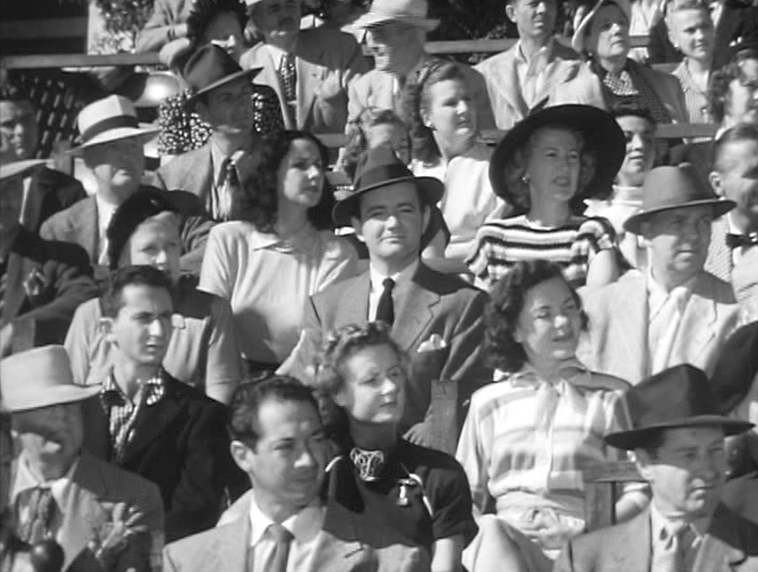
\includegraphics[width=7.5cm]{Strangers_on_a_Train.png}
\end{center}
Here, though, we observe something else; a certain sort of confusion
when a target stimulus is surrounded by distractors. In any case we
begin by thinking about the selective attention and monitoring of
contrast and similarity in visual input. In the task, originally
described in \citet{EriksenEriksen1974}, the participants are shown
one of two stimuli, here a \lq{}\textbf{S}\rq{} or a
\lq{}\textbf{H}\rq{} and they press a button in reponse, for example
left for \textbf{S} and right for \textbf{H}. The target letter is
flanked by distractors on each side the participants are told to
ignore. There are two cases, one where the distractors are compatible:
\textbf{HHH} and \textbf{SSS} and one where they are incompatible:
\textbf{HSH} and \textbf{SHS}.

Participants are slower and less accurate when responding to
incompatible flankers. This is studied from a Bayesian point of view
in \cite{YuDayanCohen2009}; they use data from older experiments in
which the participants were instructed to perform the task as quickly
as possible. One surprising and distinctive result, see
Fig.~\ref{fig_rt_accurate}, is that for very short reaction times the
response with incompatible flankers can be worse than chance. The goal
here is to understand both the error rate and the distribution of
reaction times.

\begin{figure}[tb]
\begin{center}
  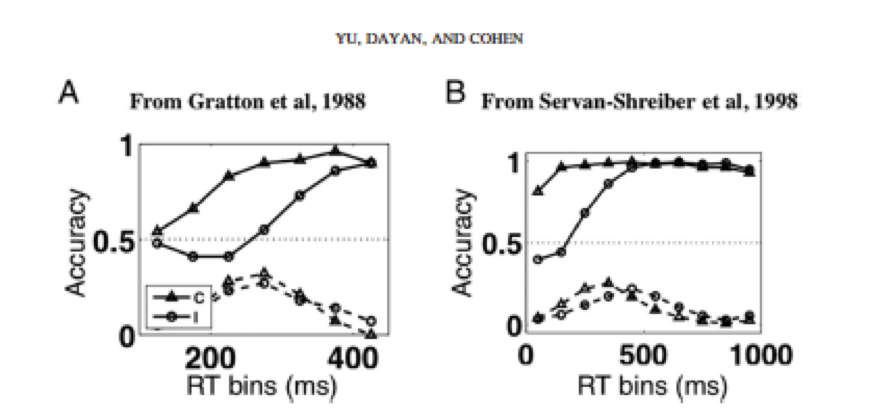
\includegraphics[width=9.5cm]{fig_rt_accurate.png}
\end{center}
\caption{The solid lines show the accuracy against reaction time; the
  dashed lines the distribution of reaction times themselves. There
  are two traces, one marked C with compatible flankers, this is
  graphed with triangles and one marked I with incompatible
  flankers. The figure was taken (by Rosalyn) from
  \cite{YuDayanCohen2009} but they themselves have adopted it from
  other studies. \label{fig_rt_accurate}}
\end{figure}

There are two hypothesis as to what is going on, the first is that
there is a compatibility bias: the brain assumes that the world is
smooth, so having \textbf{S} flankers biases it towards the
expectation that middle letter is also a \textbf{S}. This makes sense,
visual information often has a high regularity.

The second hypothesis argues that the areas of the brain that perform
high level recognition assess visual stimuli over a large receptive
field and so the recognition neurons are receiving cross talk from the
distractors.

To see if these hypotheses account for the phenomenon we will
construct a \textsl{generative model}, that is a model that could
produce fictive data with a presumed similar distribution to the real
data. Here, the generative model is a model of a neuronal response to
the stimuli. We will couple the generative model to a
\textsl{recognition model}, a model of how the brain might identify
the target, based on the information encoded in the neurons. The
recognition model describes the decision and ultimately determines
which button will be pressed; this recognition model will perform
Bayesian infernce.

Let the stimuli be labels $s_1$, $s_2$ and $s_3$, $s_2$ is the target,
$s_1$ are the letter to the left and $s_3$ to the right. In the
experiment $s_1=s_3$, in the consistient condition $s_1=s_2$, in the
inconsistient $s_1\not=s_2$. The three neurons corresponding to three
stimuli are labelled $x_1$, $x_2$ and $x_3$; these will have a
response which is different, on average, depending on which letter is
in each part of the stimulus, but they will respond in a variable
way. In fact, for definiteness, lets say the $i$th stimulus $s_i=-1$
when the letter is \textbf{S} and $s_i=1$ if it is \textbf{H}; the
$x_I$ are then Gaussian distibuted around these values. Of course, in
implementing hypothesis two, each neuron will get an input from more
than one $s_i$. The random variable $M$ describes the trial condition,
with $M=I$ for incompatible and $M=C$ for compatible. If we write
$p(M=C)=\beta$ then for hypothesis one $\beta>0.5$, whereas for
hypothesis two there is no bias so $\beta=0.5$.

If $\mu_i=\mu(s_i)$ represented the -1 or one at the $i$ letter
position corresponding to \textbf{S} and \textbf{H} we can assume a
distribution for the response, for hypothesis one this could be
\begin{equation}
p(\textbf{x}|\textbf{s})=\mathcal{N}(\mu_1,\sigma)\mathcal{N}(\mu_2,\sigma)\mathcal{N}(\mu_3,\sigma)
\end{equation}
where the $\sigma$s represent the noise in the neuronal response and the responses are assumed to be conditionally independent. For hypothesis two there is a wider receptive field so we might have
\begin{equation}
p(\textbf{x}|\textbf{s})=\mathcal{N}(t\mu_1+d\mu_2,\sigma)\mathcal{N}(d\mu_1+t\mu_2+d\mu_3,\sigma)\mathcal{N}(d\mu_2+t\mu_3,\sigma)
\end{equation}
where here the $d$ and $t$ weight the influence of the distractor and
the target on the neuronal response.

The final piece of the generator is time; the idea is that the neurons
draw repeatedly from their distribution, independently each time, so, for example:
\begin{equation}
p(\textbf{x}(t)|\textbf{s})=\mathcal{N}(\mu_1,\sigma)\mathcal{N}(\mu_2,\sigma)\mathcal{N}(\mu_3,\sigma)
\end{equation}
for all $t$. We will also treat $t$ as a discrete variable, so in this
picture the visual percept is observed for a short amount of time, say
tens of miliseconds; the neurons response to this observation and then
the cycle repeats. In reality, of course, this is a continuous
process.

Now we consider the recognition model. This assumes an \textsl{ideal
  behaviour}, that is inference based on an optimal Bayesian
strategy. In other words, given the noise in the system, the noisy
response of the neurons, the noise in the eye, the ideal observer
makes the best possible decision.

Lets imagine that the target is \textbf{H} and we are interested in
estimating $s_2$. Ultimately to calculated the probability that
$s_2=\mathbf{H}$ we will need to marginalize over the condition $M$;
but for now lets calculate $p(s_2=\mathbf{H},M=C|\textbf{x}(t))$.
Using the Bayes rule we have
\begin{equation}
p(\mathbf{H},C|\textbf{x}(t),\mbox{previous $t$})=\frac{p(\textbf{x}|\mathbf{H},C)P(\mathbf{H},C|\mbox{previous $t$})}{Z}
\end{equation}
Here $Z$ just stands for the normalization stuff on the bottom which
we won't look at closely. Clearly the clever bit is that the
recognition model is performing a Bayesian loop, updating the
posterior for time $t$ based on the previous prior and then using that
as the prior when working out time $t+1$. The distribution for
$\mathbf{x}$ conditioned on the value of the target doesn't depend on
previous results since we are assuming the generator model is time
independent; we know this distribution in that we've assumed, as
above, that it is Gaussian.

The overall idea is that the model will keep working until it reaches
a threshold $p(s_2=\mathbf{H}|\mbox{previous times})>0.9$ for example
and at that point the recognition model will call its decision.

Now at the start the prior is not based on any evidence
\begin{equation}
P(\mathbf{H},C|\mbox{at the start})=0.5\beta
\end{equation}
since at this time the condition, consistent or inconsistent, is
independent of the identity of the target, \textbf{H} or
\textbf{S}. We also have values for these quantities, we assume our
priors are $p(M=C)=\beta$, representing our expectation of consistency
and $P(s_2=\mathbf{H})=0.5$ since we have no reason to expect one over
the other. Now
\begin{equation}
p(\mathbf{H},C|\textbf{x}(1),\mbox{at the start})=\frac{0.5\beta p(\textbf{x}|\mathbf{H},C)}{Z}
\end{equation}
This gives us a posterior for time $t=1$. We would need to do the same
thing for $P(s_2=\mathbf{H},M=I|\textbf{x}(1),\mbox{at the start})$
to calculate 
\begin{equation}
P(s_2=\mathbf{H}|\textbf{x}(1),\mbox{at the
  start})
\end{equation}
If that is greater than 0.9, or less than 0.1, we stop and
declare an answer. Otherwise we iterate:
\begin{equation}
p(\mathbf{H},C|\textbf{x}(2),\textbf{x}(1),\mbox{at the start})=\frac{p(\textbf{x}|\mathbf{H},C)p(\mathbf{H},C|\textbf{x}(1),\mbox{at the start})}{Z}
\end{equation}
Clearly, although this hasn't been fleshed out in detail, it shows how
we could build a model to calculate the reaction time distribution and
the accuracy.

In \cite{YuDayanCohen2009} this is simulated for the two hypotheses. The results can be seen in Fig.~\ref{fig_h1} and Fig.~\ref{fig_h2}.
 



\begin{figure}[tb]
\begin{center}
  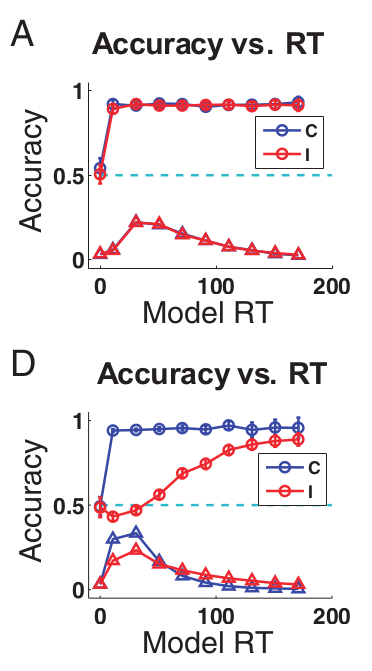
\includegraphics[width=4.5cm]{flanker_model1.png}
\end{center}
\caption{This shows the model results for the first hypothesis, with, in (\textbf{top}) $\beta=0.5$ so there is no consistency bias and (\textbf{bottom}) with $\beta=0.9$ so there is a bias. Taken from \cite{YuDayanCohen2009}. \label{fig_h1}}
\end{figure}


\begin{figure}[tb]
\begin{center}
  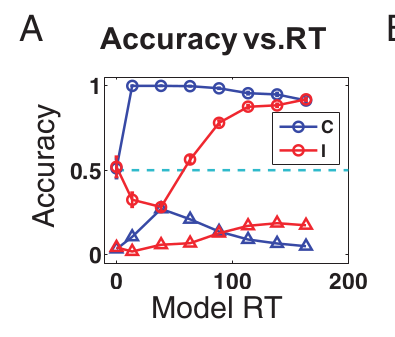
\includegraphics[width=4.5cm]{flanker_model2.png}
\end{center}
\caption{This shows the model results for the second hypothesis. Taken from \cite{YuDayanCohen2009}. \label{fig_h2}}
\end{figure}




\bibliographystyle{apa}
\bibliography{../../source/bibliography}{}



\end{document}

